% =====================================================================
% TEMPLATE ELABORASI SATU KOMPONEN
% Salin file ini menjadi komponen_NAMA.tex, lalu ganti placeholder.
% Struktur ini diselaraskan secara generik mengikuti alur dht22.tex.
% Jangan meng-input file template ini secara langsung ke bab.
% =====================================================================

\subsection{MQ-2 / MQ-135 -- Sensor Gas \& Kualitas Udara}
\label{subsec:mq_gas_sensor}

% ---------------------------------------------------------------------
\subsubsection{Identitas dan Fungsi}
\begin{wrapfigure}{r}{0.3\textwidth}% 'r' untuk posisi kanan, '0.25\textwidth' untuk lebar gambar
	\vspace{-25pt}
	\centering
	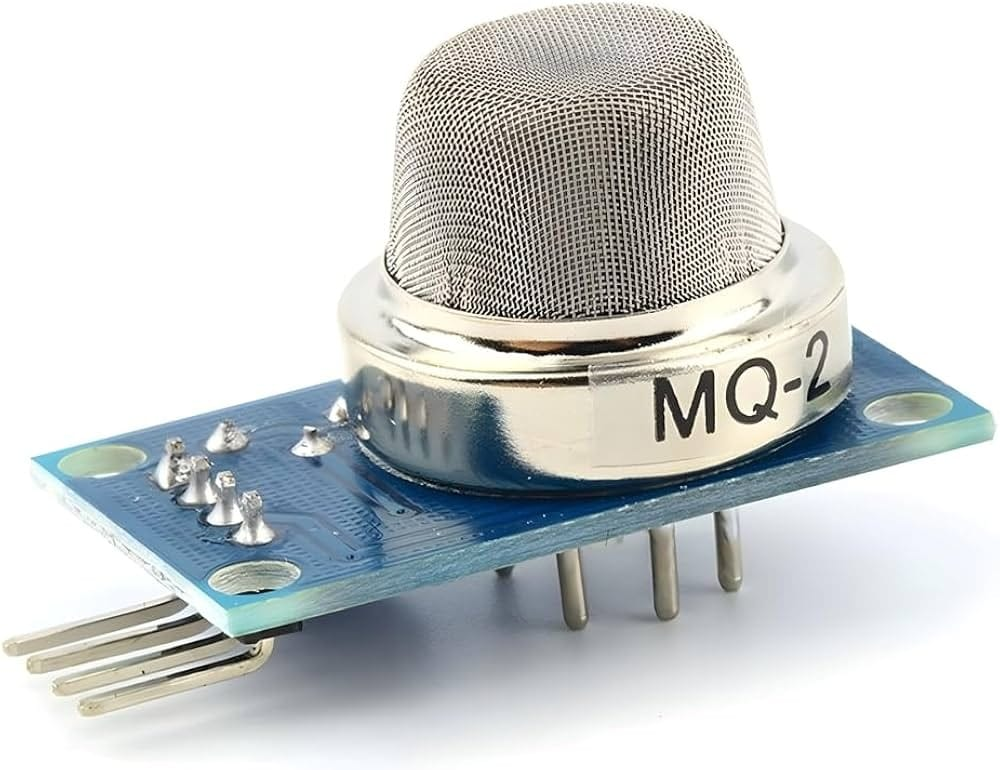
\includegraphics[width=\linewidth]{images/mq_2_gs.jpg} % Ganti dengan nama file gambar Anda
	\caption{Sensor MQ-2.}
	\label{fig:mq_gas_sensor}
\end{wrapfigure}

Sensor gas seri MQ (khususnya MQ-2 dan MQ-135) adalah modul transduser elektrokimia berbasis semikonduktor yang berfungsi untuk mendeteksi keberadaan serta mengukur konsentrasi gas spesifik di udara sekitar. Modul ini dipilih untuk dieksplorasi karena memiliki sensitivitas tinggi, rentang deteksi yang luas, waktu respons yang cepat, serta menyediakan antarmuka ganda (analog $AO$ dan digital $DO$) yang sangat mudah diintegrasikan dengan unit mikrokontroler.

\begin{itemize}
	\item \textbf{Modul MQ-2:} Difokuskan untuk deteksi kebocoran gas mudah terbakar (\textit{combustible gas}) serta asap. Sangat peka terhadap \textit{Liquefied Petroleum Gas} (LPG), propana, metana, hidrogen, serta asap pembakaran.
	\item \textbf{Modul MQ-135:} Difokuskan untuk pemantauan kualitas udara (\textit{air quality control}) ruangan/kantor. Memiliki kepekaan tinggi terhadap gas-gas beracun dan pencemar seperti amonia ($\text{NH}_3$), oksida nitrogen ($\text{NO}_x$), alkohol, benzena, asap, dan karbon dioksida ($\text{CO}_2$).
\end{itemize}

\begin{table}[H]
	\centering
	\caption{Identitas komponen Sensor Gas MQ-2 dan MQ-135}
	\label{tab:mq_identitas}
	\small
	\begin{tabularx}{\textwidth}{@{}lX@{}}
		\toprule
		Parameter          & Keterangan                                                                 \\
		\midrule
		Nama komponen      & Modul Sensor Gas Seri MQ (MQ-2 \& MQ-135)                                  \\
		Model/part number  & MQ-2 (Combustible Gas/Smoke) / MQ-135 (Air Quality/Pollutant)              \\
		Jenis              & Sensor Semikonduktor / Elektrokimia ($\text{SnO}_2$) dengan Modul Breakout \\
		Fungsi utama       & Mendeteksi konsentrasi gas terlarut ($PPM$) dan indikasi batas ambang gas  \\
		Sumber dokumentasi & Pololu Robotics \& Electronics (MQ-2) serta Olimex Ltd. (MQ-135) datasheet \\
		\bottomrule
	\end{tabularx}
\end{table}

% ---------------------------------------------------------------------
\subsubsection{Prinsip Kerja}
Sensor seri MQ beroperasi berdasarkan perubahan konduktivitas listrik pada lapisan bahan sensitif semikonduktor Timah Oksida ($\text{SnO}_2$) ketika terpapar gas target pada kondisi dipanaskan.

\begin{enumerate}
	\item \textbf{Elemen Transduser Utama ($\text{SnO}_2$ dan Elemen Pemanas):}
	      Dalam kondisi udara bersih, molekul oksigen teradsorpsi pada permukaan kristal $\text{SnO}_2$ dan menangkap elektron bebas dari pita konduksi semikonduktor, membentuk ion oksigen ($O_2^-$ atau $O^-$). Hal ini menciptakan (\textit{potential barrier}) yang menyebabkan konduktivitas bahan menjadi sangat rendah (resistansi sensor $R_s$ tinggi). Elemen pemanas internal (\textit{heater}) dari bahan kawat nikel-kromium ($R_H$) memanaskan elemen sensitif hingga suhu kerja optimal ($\approx 200\text{ s.d. }300\,^\circ\text{C}$) agar reaksi kimia permukaan dapat berlangsung secara efektif.

	      Ketika gas target yang bersifat pereduksi (\textit{reducing gas}) hadir di udara sekitar, gas tersebut bereaksi kimia dengan ion oksigen yang teradsorpsi dan melepaskan kembali elektron terperangkap ke dalam pita konduksi $\text{SnO}_2$. Akibatnya, penghalang potensial menurun dan konduktivitas bahan meningkat (resistansi $R_s$ menurun seiring tingginya konsentrasi gas).

	      \begin{figure}[H]
		      \centering
		      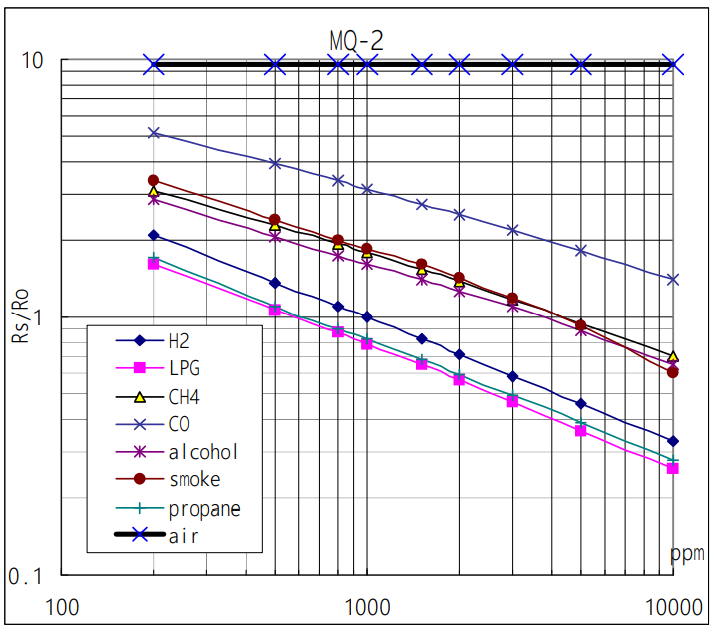
\includegraphics[width=0.5\textwidth]{images/mq_kurva.png}
		      \caption{Kurva karakteristik sensitivitas sensor MQ-2.}
		      \label{fig:mq_karakteristik}
	      \end{figure}

	\item \textbf{Elemen Pengkondisi Sinyal / Sirkuit Internal Modul:}
	      Modul \textit{breakout} memproses perubahan resistansi $R_s$ melalui dua jalur:
	      \begin{itemize}
		      \item \textbf{Jalur Analog ($AO$):} Membentuk pembagi tegangan (\textit{voltage divider}) antara resistansi sensor $R_s$ dan resistor beban $R_L$ ($10\text{ s.d. }47\,\text{k}\Omega$) untuk menghasilkan tegangan analog kontinu $V_{RL}$ yang proporsional dengan konsentrasi gas.
		      \item \textbf{Jalur Digital ($DO$):} Menggunakan IC komparator internal (seperti LM393) yang membandingkan tegangan analog $V_{RL}$ dengan tegangan acuan (\textit{threshold}) yang disesuaikan secara manual melalui potensiometer presisi (\textit{trimpot}).
	      \end{itemize}
\end{enumerate}

\begin{figure}[H]
	\centering
	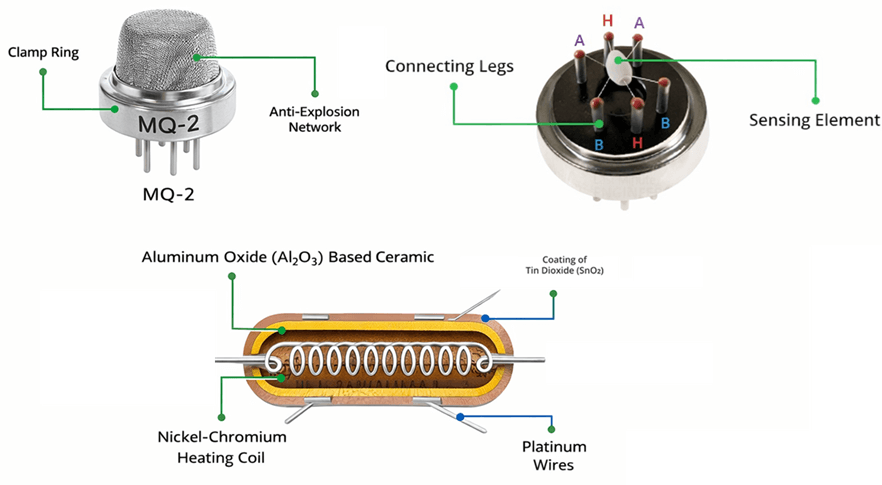
\includegraphics[width=0.75\textwidth]{images/mq-internal.png}
	\caption{Komponen internal dan elemen sensoris modul sensor MQ.}
	\label{fig:mq_internal}
\end{figure}


\paragraph{Konsep dan Formulasi Matematis Terkait}
Hubungan antara resistansi sensor $R_s$, resistansi acuan $R_0$, dan konsentrasi gas dalam \textit{Parts Per Million} ($PPM$) bersifat logaritmik dan dinyatakan melalui persamaan daya (\textit{power-law equation}):

\begin{equation}
	\frac{R_s}{R_0} = A \cdot (PPM)^b \quad \implies \quad \log\left(\frac{R_s}{R_0}\right) = b \cdot \log(PPM) + \log(A)
	\label{eq:mq_formulasi}
\end{equation}

\noindent di mana:
\begin{itemize}
	\item $R_s$ = Resistansi sensor pada berbagai konsentrasi gas target ($\Omega$).
	\item $R_0$ = Resistansi acuan sensor pada kondisi udara bersih atau konsentrasi gas standar ($\Omega$).
	\item $PPM$ = Konsentrasi gas terukur di udara (\textit{Parts Per Million}).
	\item $A, b$ = Konstanta spesifik gas target yang diperoleh dari kurva sensitivitas \textit{datasheet} (di mana $b$ mewakili kemiringan/ \textit{slope} kurva logaritmik).
\end{itemize}
% ---------------------------------------------------------------------
\subsubsection{Alur Kerja Internal dan Protokol Komunikasi}
Alur pemrosesan data modul sensor MQ mengikuti pola \textbf{Input $\rightarrow$ Proses $\rightarrow$ Output}:
\begin{enumerate}
	\item \textbf{Input:} Konsentrasi gas target di udara bereaksi dengan lapisan sensitif $\text{SnO}_2$ yang dipanaskan oleh kumparan \textit{heater} internal.
	\item \textbf{Proses:} Perubahan resistansi fisik $R_s$ diubah menjadi sinyal tegangan analog oleh sirkuit pembagi tegangan $R_L$, lalu dialirkan ke pin $AO$ sekaligus dibandingkan oleh komparator LM393 terhadap batas potensiometer.
	\item \textbf{Output:} Modul menghasilkan dua keluaran simultan berupa tegangan analog kontinu ($AO$) dan sinyal biner logika digital ($DO$).
\end{enumerate}

\paragraph{Detail Sinyal Komunikasi}
Modul sensor MQ merupakan perangkat berbasis antarmuka analog dan sakelar threshold digital, sehingga tidak menggunakan protokol transmisi serial bernavigasi clock/byte (seperti I$^2$C, SPI, atau UART).

\begin{itemize}
	\item \textbf{Inisiasi (Pemanasan Awal):} Tidak ada pulsa pemicu digital dari MCU. Namun, sensor memerlukan waktu pemanasan awal (\textit{preheat time}) selama $20\text{ s.d. }48\,\text{jam}$ untuk penggunaan awal (atau min. $3\text{ s.d. }5\,\text{menit}$ saat penyalaan rutin) agar suhu \textit{heater} stabil sebelum pembacaan valid.
	\item \textbf{Sinyal Respons :} Sinyal keluaran analog $AO$ diperbarui secara real-time dan kontinu sesuai perubahan reaksi kimia di permukaan sensor.
	\item \textbf{Format Transmisi Data:}
	      \begin{itemize}
		      \item \textbf{Jalur Analog ($AO$):} Sinyal tegangan DC kontinu ($0\text{ s.d. }5\,\text{V}$) yang dikonversi oleh ADC mikrokontroler.
		      \item \textbf{Jalur Digital ($DO$):} Sinyal TTL logika \texttt{HIGH} ($V_{CC}$) saat konsentrasi gas di bawah ambang batas, dan beralih ke \texttt{LOW} ($0\,\text{V}$) ketika konsentrasi gas melampaui batas ambang (\textbf{Active LOW}).
	      \end{itemize}

\end{itemize}

\begin{figure}[htbp]
	\centering
	\begin{tikzpicture}[x=0.18mm, y=13mm, >=Stealth, font=\sffamily\small]
		% Base axis / waktu (Sumbu vertikal ditinggikan ke 2.6)
		\draw[->, color=gray!60, thick] (0, 0) -- (600, 0) node[right, color=black] {\textit{t}};
		\draw[->, color=gray!60, thick] (0, 0) -- (0, 2.6) node[above, color=black] {$V$};

		% Level logika/tegangan Digital (Diberi offset x=-5 agar tidak menempel sumbu Y)
		\node[left, font=\scriptsize] at (-5, 1.8) {\textbf{5V ($V_{CC}$)}};
		\node[left, font=\scriptsize] at (-5, 0.4) {\textbf{0V (GND)}};
		\draw[dotted, color=gray!40] (0, 1.8) -- (580, 1.8);
		\draw[dotted, color=gray!40] (0, 0.4) -- (580, 0.4);

		% Garis Ambang Batas Analog (Threshold)
		\draw[dashed, color=red!70, thick] (0, 1.1) -- (580, 1.1) node[right, font=\scriptsize, color=red!80, align=center] {Ambang Batas \\($V_{th}$)};

		% 1. Bentuk gelombang sinyal AO (Analog Output) - Kurva Halus
		\draw[ultra thick, color=orange!80, smooth]
		plot coordinates {
				(0, 0.5) (60, 0.52) (120, 0.55) (150, 0.6)
				(180, 1.1) % Titik potong threshold naik
				(210, 1.5) (250, 1.7) (300, 1.75) (350, 1.5)
				(420, 1.1) % Titik potong threshold turun
				(450, 0.8) (500, 0.55) (600, 0.5)
			};
		% PERBAIKAN: Label AO diletakkan di bawah puncak kurva agar tidak menabrak panah atas
		\node[color=orange!90!black, font=\small\bfseries] at (300, 1.35) {AO};

		% 2. Bentuk gelombang sinyal DO (Digital Threshold)
		\draw[ultra thick, color={rgb,255:red,30;green,64;blue,175}]
		(0, 1.8) -- (180, 1.8) -- (180, 0.4) -- (420, 0.4) -- (420, 1.8) -- (600, 1.8);
		% PERBAIKAN: Label DO digeser ke kanan (x=90) dan diletakkan sedikit di bawah garis 5V
		\node[color={rgb,255:red,30;green,64;blue,175}, font=\small\bfseries] at (90, 1.55) {DO};

		% Anotasi rentang waktu (PERBAIKAN: Posisi dinaikkan ke y=2.4 agar bebas hambatan)
		\draw[stealth-stealth, color={rgb,255:red,30;green,64;blue,175}] (0, 2.4) -- (180, 2.4)
		node[midway, above, font=\scriptsize, align=center] {Kondisi Awal };
		\draw[stealth-stealth, color={rgb,255:red,217;green,119;blue,6}] (180, 2.4) -- (420, 2.4)
		node[midway, above, font=\scriptsize, align=center] { Gas > Ambang Batas};
		\draw[stealth-stealth, color={rgb,255:red,15;green,118;blue,110}] (420, 2.4) -- (600, 2.4)
		node[midway, above, font=\scriptsize, align=center] { Gas < Ambang Batas};

		% Garis bantu vertikal pembatas logika (Ditinggikan mengikuti y=2.4)
		\draw[dashed, color=gray!50] (180, 0) -- (180, 2.4);
		\draw[dashed, color=gray!50] (420, 0) -- (420, 2.4);
	\end{tikzpicture}
	\caption{Karakteristik perbandingan \textit{output} sinyal analog ($AO$) dan digital ($DO$) pada modul sensor MQ.}
	\label{fig:mq_timing_analog_digital}
\end{figure}


Pada implementasi praktis mikrokontroler, pembacaan sinyal analog $AO$ dikonversi oleh periferal ADC internal, lalu program (atau pustaka komponen spesifik sensor) bertugas mentranslasi sinyal tersebut ke nilai konsenstrasi gas ($PPM$).

% ---------------------------------------------------------------------
\subsubsection{Besaran yang Diukur atau Dikendalikan}
Sensor seri MQ mengukur konsentrasi gas terlarut di udara sekitar yang dinyatakan dalam satuan \textit{Parts Per Million} ($PPM$). Masing-masing sensor (MQ-2 dan MQ-135) memiliki rentang sensitivitas dan tingkat respon yang berbeda-beda terhadap jenis gas target spesifik.

\begin{table}[H]
	\centering
	\caption{Karakteristik besaran dan rentang deteksi gas spesifik komponen MQ-2 dan MQ-135}
	\label{tab:mq_karakteristik_besaran}
	\small
	\begin{tabularx}{\textwidth}{@{} p{2.4cm} l X X @{}}
		\toprule
		Parameter               & Model                                         & Nilai / Gas Target                                     & Keterangan                                     \\
		\midrule
		Besaran Utama           & MQ-2 / MQ-135                                 & Konsentrasi Gas ($PPM$)                                & Pengukuran kepekaan gas di atmosfer            \\
		\midrule
		\multirow{10}{*}{\parbox{2.2cm}{\textbf{Rentang Kerja Gas Spesifik}}}
		                        & \multirow{5}{*}{MQ-2}
		                        & LPG: $200\text{ s.d. }5000\,\text{ppm}$           & Gas elpiji / propana-butana                                                                             \\
		                        &                                               & Propana ($C_3H_8$): $200\text{ s.d. }5000\,\text{ppm}$     & Gas hidrokarbon mudah terbakar                 \\
		                        &                                               & Hidrogen ($H_2$): $300\text{ s.d. }5000\,\text{ppm}$       & Gas terbakarnya industri                       \\
		                        &                                               & Metana ($CH_4$): $500\text{ s.d. }2000\,\text{ppm}$        & Gas alam / rawa                                \\
		                        &                                               & Asap / Alkohol: $200\text{ s.d. }2000\,\text{ppm}$         & Partikel pembakaran \& uap organik             \\
		\cmidrule{2-4}
		                        & \multirow{5}{*}{MQ-135}
		                        & Amonia ($NH_3$): $10\text{ s.d. }300\,\text{ppm}$ & Pencemar gas limbah / buangan                                                                           \\
		                        &                                               & Benzena ($C_6H_6$): $10\text{ s.d. }1000\,\text{ppm}$      & Senyawa volatil hidrokarbon                    \\
		                        &                                               & Alkohol: $10\text{ s.d. }300\,\text{ppm}$                  & Uap pelarut / alkohol murni                    \\
		                        &                                               & Karbon Dioxida ($CO_2$): $10\text{ s.d. }1000\,\text{ppm}$ & Pemantauan kualitas udara ruangan              \\
		                        &                                               & Asap / $NO_x$: $10\text{ s.d. }1000\,\text{ppm}$           & Gas sisa pembakaran kendaraan                  \\
		\midrule
		Resolusi                & MQ-2 / MQ-135                                 & Kontinu (Analog)                                       & Bergantung pada resolusi ADC MCU (mis. 10-bit) \\
		Sensitivitas ($S$)      & MQ-2 / MQ-135                                 & $R_s(\text{gas}) / R_s(\text{udara bersih}) \ge 5$     & Rasio perubahan hambatan $R_s$ di udara        \\
		Waktu Respons ($t_r$)   & MQ-2 / MQ-135                                 & $\le 10\,\text{s}$                                     & Tanggapan terhadap kenaikan konsentrasi        \\
		Waktu Pemulihan ($t_h$) & MQ-2 / MQ-135                                 & $\le 30\,\text{s}$                                     & Waktu pembersihan elemen sensor                \\
		\bottomrule
	\end{tabularx}
\end{table}

% ---------------------------------------------------------------------
\subsubsection{Karakteristik Sinyal}
Keluaran sinyal dari modul MQ disesuaikan dengan kebutuhan pemrosesan pada mikrokontroler.

\begin{equation}
	V_{OUT}(AO) = V_{CC} \times \left( \frac{R_L}{R_s + R_L} \right)
	\label{eq:mq_packet}
\end{equation}

\begin{table}[H]
	\centering
	\caption{Karakteristik sinyal modul MQ-2 / MQ-135}
	\label{tab:mq_sinyal}
	\small
	\begin{tabularx}{\textwidth}{@{}lXX@{}}
		\toprule
		Aspek                      & Nilai                                           & Keterangan                                                 \\
		\midrule
		Jenis sinyal               & Analog Tegangan DC ($AO$) \& Digital TTL ($DO$) & Antarmuka ganda (\textit{dual output})                     \\
		Level logika $DO$          & TTL $0\,\text{V}$ / $5\,\text{V}$               & Active \texttt{LOW} ketika gas melampaui ambang batas      \\
		Rentang tegangan $AO$      & $0{,}1\text{ s.d. }4{,}5\,\text{V DC}$              & Berbanding lurus dengan konsentrasi gas                    \\
		Frekuensi / Kecepatan Data & Kontinu (Real-time)                             & Dibatasi oleh waktu respon sensor ($\approx 10\,\text{s}$) \\
		Respons Komponen           & Perubahan Tegangan $AO$                         & Berubah seiring dinamika konsentrasi gas                   \\
		Format Data / Encoding     & Rasio Tegangan Analog                           & Perlu dikonversi melalui fungsi ADC MCU                    \\
		\bottomrule
	\end{tabularx}
\end{table}

% ---------------------------------------------------------------------
\subsubsection{Pin, Catu Daya, dan Antarmuka}
Modul sensor MQ umumnya dikemas dalam bentuk modul \textit{breakout} 4-pin yang sudah mengintegrasikan sensor MQ 6-pin mentah, resistor beban $R_L$, potensiometer kalibrasi, serta IC komparator LM393.

\begin{figure}[H]
	\centering
	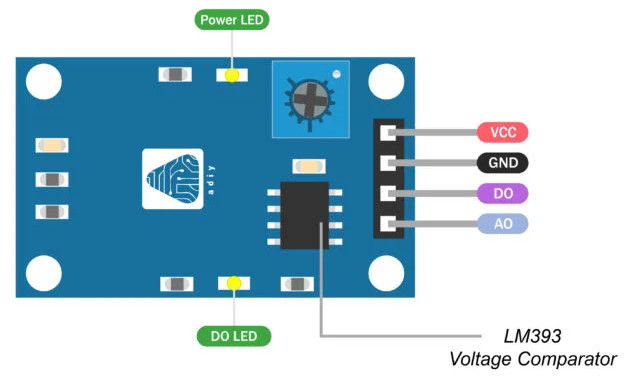
\includegraphics[width=0.5\textwidth]{images/mq-2_pinout.jpg}
	\caption{Pemetaan pin dan antarmuka modul sensor MQ.}
	\label{fig:mq_pinout}
\end{figure}

\begin{table}[H]
	\centering
	\caption{Pemetaan pin dan antarmuka modul breakout MQ-2 / MQ-135}
	\label{tab:mq_pin}
	\small
	\begin{tabularx}{\textwidth}{@{}llX@{}}
		\toprule
		Pin (Modul Breakout) & Fungsi   & Keterangan                                                \\
		\midrule
		VCC / VIN            & $V_{CC}$ & Daya Pemanas ($V_H$) \& Sirkuit ($V_C$) $+5\,\text{V DC}$ \\
		AOUT / AO            & Sinyal   & Keluaran Tegangan Analog ke ADC MCU                       \\
		DOUT / DO            & Kontrol  & Keluaran Digital Threshold (Komparator LM393)             \\
		GND                  & GND      & Referensi ground sistem ($0\,\text{V}$)                   \\
		\bottomrule
	\end{tabularx}
\end{table}

\subsubsection{Kebutuhan Catu Daya}
Modul sensor MQ membutuhkan catu daya yang teratur dan presisi sebesar $5{,}0\,\text{V DC} \pm 0{,}1\,\text{V}$. Elemen pemanas internal ($R_H$) mengonsumsi arus yang lumayan besar untuk ukuran sensor, yaitu berkisar $150\text{ s.d. }180\,\text{mA}$ dengan konsumsi daya hingga $\le 800\text{ s.d. }900\,\text{mW}$.

Oleh karena itu, modul ini sangat tidak disarankan diberi catu daya langsung dari pin luaran regulator $5\,\text{V}$ mikrokontroler berkapasitas rendah untuk menghindari penurunan tegangan (\textit{brownout}). Pemasangan kapasitor \textit{decoupling} $100\,\text{nF}$ secara paralel antara pin $V_{CC}$ dan GND sangat direkomendasikan guna menekan fluktuasi tegangan. Modul ini bekerja pada level logika $5\,\text{V}$ TTL; jika dihubungkan ke mikrokontroler berbasis $3{,}3\,\text{V}$ (seperti ESP32/STM32), pin $AO$ memerlukan pembagi tegangan (\textit{voltage divider}) eksternal agar tidak merusak pin ADC MCU.

% ---------------------------------------------------------------------
\subsubsection{Spesifikasi Penting dari Datasheet}

\begin{table}[H]
	\centering
	\caption{Spesifikasi penting modul sensor gas MQ-2 dan MQ-135}
	\label{tab:mq_spesifikasi}
	\small
	\begin{tabularx}{\textwidth}{@{}Xc@{}}
		\toprule
		Parameter                                     & Nilai                                                                                      \\
		\midrule
		Tegangan Kerja Sirkuit ($V_C$)                & $5{,}0 \pm 0{,}1$ $\text{V DC}$                                                            \\
		Tegangan Pemanas ($V_H$)                      & $5{,}0 \pm 0{,}1$ $\text{V DC}$                                                            \\
		Resistansi Pemanas ($R_H$) -- \textbf{MQ-2}   & $31 \pm 3$ $\Omega$                                                                        \\
		Resistansi Pemanas ($R_H$) -- \textbf{MQ-135} & $33 \pm 5\%$ $\Omega$                                                                      \\
		Konsumsi Daya Pemanas ($P_H$)                 & $\le 800 \text{ s.d. } 900$ $\text{mW}$                                                        \\
		Resistansi Sensor ($R_s$) -- \textbf{MQ-2}    & $2 \text{ s.d. } 20$ (pada $2000\,\text{ppm}$ Isobutana) $\text{k}\Omega$                      \\
		Resistansi Sensor ($R_s$) -- \textbf{MQ-135}  & $30 \text{ s.d. } 200$ (pada $100\,\text{ppm} \; \text{NH}_3/\text{Alkohol}$) $\text{k}\Omega$ \\
		Suhu Operasional Lingkungan                   & $-10 \text{ s.d. } +50$ $^\circ\text{C}$                                                   \\
		\bottomrule
	\end{tabularx}
\end{table}

% ---------------------------------------------------------------------
\subsubsection{Koneksi dengan Mikrokontroler dan Implementasi Kode}
Modul sensor gas seri MQ dihubungkan ke mikrokontroler target Arduino Mega 2560 (ATmega2560) dengan memanfaatkan dua jenis periferal internal utama: kanal ADC  10-bit untuk membaca tingkat konsentrasi gas secara kontinu melalui sinyal analog $AO$, serta modul \textbf{External Interrupt / GPIO Digital} untuk membaca sinyal batas $DO$ dari komparator LM393 secara \textit{real-time}.

\paragraph{Rangkaian Skematik dan Simulasi}
Pengujian antarmuka perangkat keras dapat divalidasi melalui simulator daring (seperti Wokwi) maupun perakitan *breadboard* secara fisik:
\begin{itemize}
	\item \textbf{Koneksi Catu Daya:} Pin VCC modul MQ dihubungkan ke rel daya $5\,\text{V}$ eksternal atau pin $5\text{V}$ Arduino Mega 2560 untuk memberi pasokan daya elemen pemanas internal ($R_H$) dan sirkuit komparator. Pin GND dihubungkan ke \textit{ground} sistem bersama (\textit{common ground}).
	\item \textbf{Koneksi Sinyal dan Komponen Pasif:} Pin keluaran analog $AO$ dihubungkan ke kanal ADC \texttt{A0} (PF0) mikrokontroler. Pin keluaran digital $DO$ dihubungkan ke GPIO pin 2 Digital pada Mega 2560 yang mendukung fungsi interupsi eksternal (\texttt{INT4}). Resistor pembagi tegangan eksternal tidak diperlukan karena modul \textit{breakout} MQ telah mengintegrasikan resistor beban $R_L$ ($10\text{ s.d. }47\,\text{k}\Omega$) dan komparator LM393.
\end{itemize}

\begin{figure}[htbp]
	\centering
	% Ganti dengan file skematik rangkaian aktual atau tangkapan layar simulasi Wokwi
	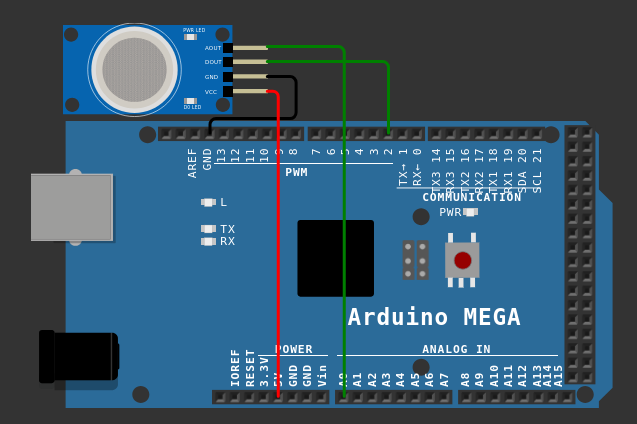
\includegraphics[width=0.70\textwidth]{images/mq_wokwi_diagram.png}
	% \fbox{\parbox[c][5cm][c]{0.70\textwidth}{\centering Tempatkan tangkapan layar simulasi Wokwi atau diagram skematik antarmuka Sensor MQ dengan Arduino Mega 2560 di sini}}
	\caption{Rangkaian demonstrasi sensor MQ-2 / MQ-135 dengan Arduino Mega 2560 pada simulasi wokwi.}
	\label{fig:mq_sensor_schematic}
\end{figure}

Rincian pemetaan koneksi fisik antara pin modul MQ dan fungsi periferal mikrokontroler Arduino Mega 2560 dirangkum pada Tabel~\ref{tab:mq_mcu_mapping}.

\begin{table}[H]
	\centering
	\caption{Pemetaan antarmuka modul sensor MQ ke mikrokontroler Arduino Mega 2560}
	\label{tab:mq_mcu_mapping}
	\small
	\begin{tabularx}{\textwidth}{@{}p{5.0cm}XX@{}}
		\toprule
		Kebutuhan Komponen            & Fitur MCU                                         & Alasan Pemilihan \& Fungsi                                                                                                 \\
		\midrule
		Pembacaan Konsentrasi $AO$    & ADC 10-bit (\texttt{A0})                          & Konversi tegangan analog kontinu ($0\text{ s.d. }5\,\text{V}$) menjadi nilai digital ($0\text{ s.d. }1023$) untuk kalkulasi $PPM$. \\
		Deteksi Ambang Bahaya $DO$    & Interupsi Eksternal (Pin 2)                       & Memicu penanganan interupsi (\textit{ISR}) secara instan saat kondisi gas melampaui batas (\textbf{Active LOW}).           \\
		Daya Elemen Pemanas ($R_H$)   & Rel Catu Daya $5\,\text{V DC}$ ($180\,\text{mA}$) & Menyediakan daya pemanas stabil agar elemen sensitif $\text{SnO}_2$ mencapai suhu kerja optimal.                           \\
		Pencegahan Kondisi Mengambang & Komparator LM393 Internal Modul                   & Memastikan perubahan sinyal logika $DO$ tegas (
		\textit{clean TTL}) tanpa fluktuasi saat di ambang batas.                                                                                                                                                      \\
		\bottomrule
	\end{tabularx}
\end{table}

\paragraph{Kode Demo Pengujian}
Berikut adalah contoh implementasi program C++ minimal pada mikrokontroler Arduino Mega 2560 untuk membaca data analog $AO$ (beserta kalkulasi rasio tegangan) dan menangani sinyal bahaya digital $DO$ menggunakan \textbf{Interrupt Service Routine} (ISR):

\begin{lstlisting}[language=C++, caption={Kode program pengujian Sensor MQ-2 / MQ-135 pada Arduino Mega 2560}, label={lst:mq_code}]
#define MQ_ANALOG_PIN  A0;
#define MQ_DIGITAL_PIN 2;

volatile bool gasTerdeteksi = false;

void ISR_GasDetected() {
  gasTerdeteksi = (digitalRead(MQ_DIGITAL_PIN) == LOW);
}

void setup() {
  Serial.begin(9600);

  while (!Serial) { ; }
  Serial.println(F(" Inisialisasi Pengujian Sensor Seri MQ  "));

  pinMode(MQ_DIGITAL_PIN, INPUT_PULLUP);
  attachInterrupt(digitalPinToInterrupt(MQ_DIGITAL_PIN), ISR_GasDetected, CHANGE);

  Serial.println(F("Melakukan Pre-heating Sensor (Tunggu Stabil)..."));

  delay(2000);

  Serial.println(F("Sensor Siap."));
}

void loop() {
  int rawADC = analogRead(MQ_ANALOG_PIN);
  float voltage = (rawADC / 1023.0) * 5.0;
  Serial.print(F("Nilai ADC: "));
  Serial.print(rawADC);
  Serial.print(F(" | Tegangan AO: "));
  Serial.print(voltage, 2);
  Serial.print(F(" V | Status Digital DO: "));

  if (gasTerdeteksi) {
    Serial.println(F("BAHAYA! (Gas > Threshold)"));
  } else {
    Serial.println(F("Aman / Normal"));
  }
  delay(1000);
}
\end{lstlisting}

\paragraph{Gambaran Hasil Pembacaan}
Setelah kode diunggah ke mikrokontroler atau dijalankan melalui simulasi Wokwi, keluaran pembacaan data pada \textit{Serial Monitor} akan tampak seperti pada contoh log berikut:

\begin{verbatim}
Inisialisasi Pengujian Sensor Seri MQ
Melakukan Pre-heating Sensor (Tunggu Stabil)...
Sensor Siap.
Nilai ADC: 907 | Tegangan AO: 4.43 V | Status Digital DO: Aman / Normal
Nilai ADC: 973 | Tegangan AO: 4.76 V | Status Digital DO: BAHAYA!
(Gas > Threshold)
Nilai ADC: 816 | Tegangan AO: 3.99 V | Status Digital DO: Aman / Normal
\end{verbatim}
